\chapter{Design Examples} \label{ch:DesignExamples}
\chapterquote{Love does not grown on trees or brought in the market, but if one wants to be “Loved” one must first know how to give unconditional Love.}{Kabeer}

\graphicspath{{Chapters/DesignExamples/Figures/}}
\lstinputpath{Codes-Verilog/Chapter-Design-Examples} %path is defined in mypreamble


\section{Introduction}
In previous chapters, some simple designs were introduces e.g. mod-m counter and flip-flops etc. to introduce the Verilog programming. In this chapter various examples are added, which can be used to implement or emulate a system on the FPGA board. 

All the design files are provided inside the `VerilogCodes' folder inside the main project directory; which can be used to implement the design using some other software as well. Each section shows the list of Verilog-files require to implement the design in that section. Lastly, all designs are tested using \textbf{Modelsim} and on \textbf{Altera-DE2 FPGA board}. Set the desired design as `top-level entity' to implement or simulate it. 

\section{Random number generator}
In this section, random number generator is implemented using linear feedback shift register. Verilog files required for this example are listed below, 
\begin{enumerate}
	\item rand\_num\_generator.v
	\item rand\_num\_generator\_visualTest.v
	\item clockTick.v
	\item modMCounter.v
\end{enumerate}
Note that, `clockTick.v' and `modMCounter.v' are discussed in Chapter \ref{ch:VisualVerification}.

\subsection{Linear feedback shift register (LFSR)}
Long LFSR can be used as `\textbf{pseudo-random number generator}'.  These random numbers are generated based on initial values to LFSR. The sequences of random number can be predicted if the initial value is known. However, if LFSR is quite long (i.e. large number of initial values are possible), then the generated numbers can be considered as random numbers for practical purposes.  

LFSR polynomial are written as \textbf{${{\mathbf{x}}^{\mathbf{3}}}{\mathbf{ + }}{{\mathbf{x}}^{\mathbf{2}}}{\mathbf{ + 1}}$}, which indicates that the feedback is provided through output of `\textbf{xor}' gate whose  inputs are connected to positions \textbf{3}, \textbf{2} and \textbf{0} of LFSR. Some of the polynomials are listed in Table \ref{tbl:polynomial}.


\begin{table}[!h]
	\centering
	\caption{List of feedback polynomials}
	\label{tbl:polynomial}
	\begin{tabular} {|c |c |}
		\hline
		\textbf{Number of bits} & \textbf{Feedback polynomial} \\ \hline
		3    & ${x^3} + {x^2} + 1$ \\ \hline
		4    & ${x^4} + {x^3} + 1$ \\ \hline
		5    & ${x^5} + {x^3} + 1$ \\ \hline
		6    & ${x^6} + {x^5} + 1$ \\ \hline
		7    & ${x^7} + {x^6} + 1$ \\ \hline
		9    & ${x^9} + {x^5} + 1$ \\ \hline
		10   & ${x^{10}} + {x^7} + 1$ \\ \hline
		11   & ${x^{11}} + {x^9} + 1$ \\ \hline
		15   & ${x^{15}} + {x^{14}} + 1$ \\ \hline
		17   & ${x^{17}} + {x^{14}} + 1$ \\ \hline
		18   & ${x^{18}} + {x^{11}} + 1$ \\ \hline
	\end{tabular}
\end{table}

Random numbers are generated using LFSR in Listing \ref{verilog:rand_num_generator}. The code implements the design for 3 bit LFSR, which can be modified for LFSR with higher number of bits as shown below,  
\begin{explanation}[Listing \ref{verilog:rand_num_generator}]
	The listing is currently set according to 3 bit LFSR i.e. N = 3 in Line 12.  `q' is the output of LFSR, which is random in nature. Lines 26-35 sets the initial value for LFSR to 1 during reset operations. Note that, LFSR can not have `0' as initial values. Feedback polynomial is implemented at Line 43. Line 55 shifts the last N bits (i.e. N to 1) to the right by 1 bit and the $N^{th}$ bit is feed with `feedback\_value' and stored in `r\_next' signal. In next clock cycle, value of r\_next is assigned to r\_reg through Line 34. Lastly, the value r\_reg is available to output port from Line 56.
	
	Simulation results are shown in Fig. \ref{fig:rand_num_generator}. Here, we can see that total 7 different numbers are generated by LFSR, which can be seen between two cursors in the figure.  Further, q values are represented in `hexadecimal format' which are same as r\_reg values in `binary format'. 
	
	\textbf{Note that, in Fig. \ref{fig:rand_num_generator}, the generated sequence contains `8, C, 6, B, 5, 2 and 1'; and if we initialize the system with any of these values, outputs will contain same set of numbers again. If we initialize the system with `3' (which is not the set), then the generate sequence will be entirely different.}
	
	\begin{figure}[!h]
		\centering
		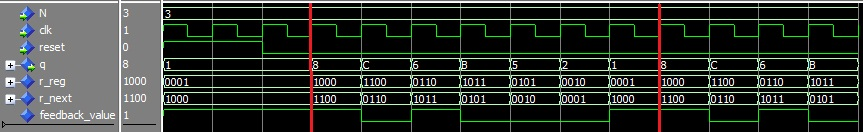
\includegraphics[width=\textwidth]{rand_num_generator}
		\caption{Random number generation with N = 3}
		\label{fig:rand_num_generator}
	\end{figure}
	
	To modify the feedback polynomial, first insert the correct number of bits (i.e. N) in  Line 12. Next, modify the feedback\_value at line 43, according to new value of `N'.\textbf{ Note that maximum-length for a polynomial is defined as $2^N-1$, but not all the polynomials generate maximum length; e.g. N = 5 generates total 28 sequences (not 31) before repetition as shown in Fig. \ref{fig:rand_num_generatorN5}. }
	
	\begin{figure}[!h]
		\centering
		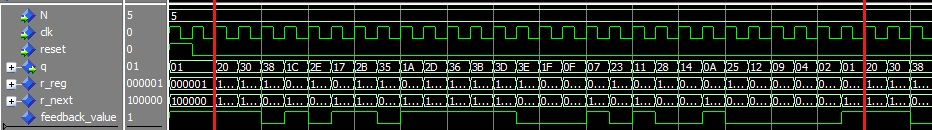
\includegraphics[width=\textwidth]{rand_num_generatorN5}
		\caption{Total sequences are 28 (not 31) for N = 5}
		\label{fig:rand_num_generatorN5}
	\end{figure}
\end{explanation}


\lstinputlisting[
language = Verilog,
caption    = {Random number generation with LFSR},
label      = {verilog:rand_num_generator}
]{rand_num_generator.v}

\subsection{Visual test}
Listing \ref{verilog:rand_num_generator_visualTest} can be used to test the Listing \ref{verilog:rand_num_generator} on the FPGA board. Here, 1 second clock pulse is used to visualize the output patterns. Please read Chapter \ref{ch:VisualVerification} for better understanding of the listing. Note that,  N = 3 is set in Line 13 according to Listing \ref{verilog:rand_num_generator}.

For displaying outputs on FPGA board, set reset to 1 and then to 0. Then LEDs will blink to display the generated bit patterns by LFSR; which are shown in Fig. \ref{fig:rand_num_generator}. 

\lstinputlisting[
language = Verilog,
caption    = {Visual test : Random number generation with LFSR},
label      = {verilog:rand_num_generator_visualTest}
]{rand_num_generator_visualTest.v}


\section{Shift register}
Shift register are the registers which  are used to shift the stored bit in one or both directions. In this section, shift register is implemented which can be used for shifting data in both direction. Further it can be used as parallel to serial converter or serial to parallel converter. Verilog files required for this example are listed below, 
\begin{enumerate}
	\item shift\_register.v
	\item shift\_register\_visualTest.v
	\item clockTick.v
	\item modMCounter.v
	\item parallel\_to\_serial.v
	\item serial\_to\_parallel.v
	\item parallel\_and\_serial\_top.v
	\item parallel\_and\_serial\_top\_visual.v
\end{enumerate}
Note that, `clockTick.v' and `modMCounter.v' are discussed in Chapter \ref{ch:VisualVerification}.

\subsection{Bidirectional shift register}
Listing \ref{verilog:shift_register} implements the bidirectional shift register which is explained below, 

\begin{explanation}[Listing \ref{verilog:shift_register}]
	In the listing, the `ctrl' port is used for `shifting', `loading' and `reading' data operation. Lines 28 clear the shift register during reset operation, otherwise go to the next state. 
	
	Lines 35-40 perform various operations based on `ctrl' values. Note that, to perform right shift (Line 37), data is continuously provided from last port i.e. (data(N-1)); whereas for left shift (Line 38) data is provided from first port i.e. (data(0)). 
	
	Next, ctrl=``00'' is provided for reading the data. It can be used for serial to parallel conversion i.e. when all the bits are shifted and register is full; then set ctrl to ``00'' and read the data, after that set ctrl to ``01'' or ``10'' for getting next set of bits. 
	
	Similarly, for parallel to serial converter, first load the data using ctrl=``11''; and then perform the shift operation until all the bits are read and then again load the data. Note that, in this case, last bit propagates (i.e. data(N-1) for right shift or data(0) for left shift) during shifting; which is actually designed for serial to parallel converter. But this will affect the working of parallel to serial converter, as we will set ctrl to ``11'', when all the data is shifted, therefore all the register which were filled by values from last port, will be overwritten by the new parallel data. 
	
	Lastly, data is available on the output port `q\_reg' from Line 43. For, parallel to serial converter, use only one pin of `q\_reg' i.e. q\_reg(0) for right shift or q(N-1) for left shift; whereas for serial to parallel conversion, complete  `q\_reg' should be read.
	
	Fig. \ref{fig:shift_register} shows the shifting operation performed by the listing. Here first data ( i.e. 00110000) is loaded with ctrl=``11''. Then shifted to right after first cursor and later to the left i.e. after second cursor.
	
	\begin{figure}[!h]
		\centering
		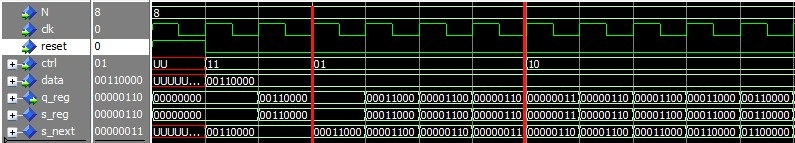
\includegraphics[width=\textwidth]{shift_register}
		\caption{Right and left shifting operations}
		\label{fig:shift_register}
	\end{figure}	 
\end{explanation}

\lstinputlisting[
language = Verilog,
caption    = {Bidirectional shift register},
label      = {verilog:shift_register}
]{shift_register.v}

\subsection{Visual test}

Listing \ref{verilog:shift_register_visualTest} can be used to test the Listing \ref{verilog:shift_register} on the FPGA board. Here, 1 second clock pulse is used to visualize the output patterns. Here, outputs (i.e. q\_reg) are displayed on LEDR; whereas `shifting-control (i.e. ctrl)' and data-load (i.e. data) operations are performed using SW[16:15] and SW[7:0] respectively. Here, we can see the shifting of LEDR pattern twoards right or left based on SW[16:15] combination. Please read Chapter \ref{ch:VisualVerification} for better understanding of the listing.

\lstinputlisting[
language = Verilog,
caption    = {Visual test : bidirectional shift register},
label      = {verilog:shift_register_visualTest}
]{shift_register_visualTest.v}

\subsection{Parallel to serial converter}
If data is loaded first (i.e. ctrl = ``11''), and later shift operation is performed (i.e.. ctrl = ``01'' or ``10''); then Listing \ref{verilog:shift_register} will work as `parallel to serial converter'. Listing \ref{verilog:parallel_to_serial} performs the conversion operation, which is tested in Section \ref{sec:testPS}. Please read comments for further details.

\lstinputlisting[
language = Verilog,
caption    = {Parallel to serial conversion},
label      = {verilog:parallel_to_serial}
]{parallel_to_serial.v}


\subsection{Serial to parallel converter}
If shifting is performed first (i.e.. ctrl = ``01'' or ``10''), and later data is read (i.e. ctrl = ``00''); then Listing \ref{verilog:serial_to_parallel} will work as `serial to parallel converter'. Listing \ref{verilog:parallel_to_serial} performs the conversion operation, which is tested in Section \ref{sec:testPS}. Please read comments for further details.

\lstinputlisting[
language = Verilog,
caption    = {Serial to parallel conversion},
label      = {verilog:serial_to_parallel}
]{serial_to_parallel.v}

\subsection{Test for Parallel/Serial converters} \label{sec:testPS}
Here, 4-bit count (i.e. parallel data) is generated using Mod-12 counter. This data is converted into serial data by Listing \ref{verilog:parallel_to_serial}; and sent to Listing \ref{verilog:serial_to_parallel}, where data is again converted into parallel and the result (i.e. count) is displayed at output as shown in Listing \ref{verilog:parallel_and_serial_top}. The simulation results are shown in Fig. \ref{fig:parallel_and_serial_top}. Lastly, visual verification circuit is shown in Listing \ref{verilog:parallel_and_serial_top_visual}. \textbf{Note that, empty\_tick signal is used as clock for modMCounter (see red line in Fig. \ref{fig:parallel_and_serial_design}), so that next count will be available when previous conversion is completed}. Please read comments for further details.
\begin{figure}[!h]
	\centering
	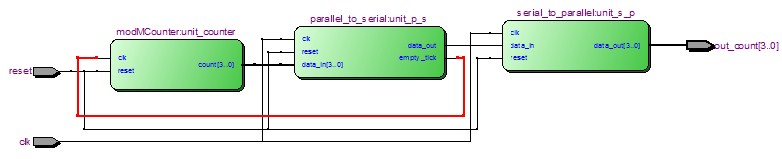
\includegraphics[width=\textwidth]{parallel_and_serial_design}
	\caption{RTL view of Listing \ref{verilog:parallel_and_serial_top}}
	\label{fig:parallel_and_serial_design}
\end{figure}

\lstinputlisting[
language = Verilog,
caption    = {Test for Parallel/Serial converters (results are in Fig. \ref{fig:parallel_and_serial_top})},
label      = {verilog:parallel_and_serial_top}
]{parallel_and_serial_top.v}

\begin{figure}[!h]
	\centering
	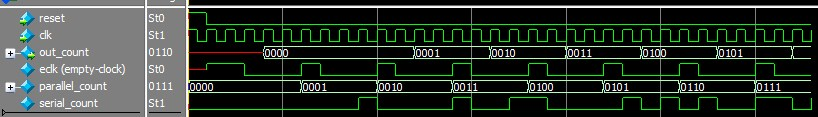
\includegraphics[scale=0.8]{parallel_and_serial_top}
	\caption{Simulation results of Listing \ref{verilog:parallel_and_serial_top}}
	\label{fig:parallel_and_serial_top}
\end{figure}

\lstinputlisting[
language = Verilog,
caption    = {Visual test for Parallel/Serial converters},
label      = {verilog:parallel_and_serial_top_visual}
]{parallel_and_serial_top_visual.v}

\section{Random access memory (RAM)}
RAM is memory cells which are used to store or retrieve the data. Further, FPGA chips have separate RAM modules which can be used to design memories of different sizes and types, as shown in this section. Verilog files required for this example are listed below, 
\begin{enumerate}
	\item single\_port\_RAM.v
	\item single\_port\_RAM\_visualTest.v
	\item dual\_port\_RAM.v
	\item dual\_port\_RAM\_visualTest.v
\end{enumerate}

\subsection{Single port RAM}
Single port RAM has one input port (i.e. address line) which is used for both storing and retrieving the data, as shown in Fig. \ref{fig:single_port_RAM}. Here `addr[1:0]' port is used for both `read' and `write' operations. Listing \ref{verilog:single_port_RAM} is used to generate this design. 
\begin{figure}[!h]
	\centering
	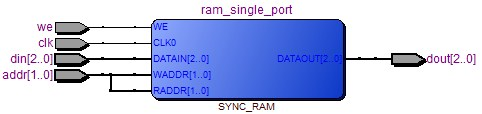
\includegraphics[scale=0.8]{single_port_RAM}
	\caption{RTL view : Single port RAM (Listing \ref{verilog:single_port_RAM})}
	\label{fig:single_port_RAM}
\end{figure}

\begin{explanation}[Listing \ref{verilog:single_port_RAM}]
	In the listing port `addr' (Line 23) is 2 bit wide as `addr\_width' is set to 2 (Line 17). Therefore, total `4 elements (i.e. $2^2$)' can be stored in the RAM. Further, `din' port (Line 24) is 3 bit wide as `data\_width' is set to 3 (Line 18); which means the data should be 3 bit wide. \textbf{In summary, current RAM-designs can store `4 elements' in it and each elements should be 3-bit wide (see declaration at Line 28 as well).}
	
	Write enable (we) port should be high and low for storing and retrieving the data respectively. `din' port is used to write the data in the memory; whereas `dout' port is used for reading the data from the memory. In Lines 32-33, the write operation is performed on rising edge of the clock; whereas read operation is performed at Line 37. 
	
	
	
	Lastly, Fig. \ref{fig:single_port_RAM_Wave} shows the simulation results for the design. Here, `we' is set to 1 after first cursor and the data is written at three different addresses (not 4). Next, `we' is set to 0 after second cursor and read operations are performed for all addresses. Since, no values is stored for address `10', therefore dout is displayed as `UUU' for this address as shown after third cursor. 
	\begin{figure}[!h]
		\centering
		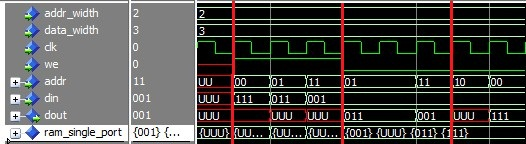
\includegraphics[scale=0.75]{single_port_RAM_Wave}
		\caption{Simulation results : Single port RAM (Listing \ref{verilog:single_port_RAM})}
		\label{fig:single_port_RAM_Wave}
	\end{figure}
\end{explanation}

\lstinputlisting[
language = Verilog,
caption    = {Single port RAM},
label      = {verilog:single_port_RAM}
]{single_port_RAM.v}

\subsection{Visual test : single port RAM}
Listing \ref{verilog:single_port_RAM_visualTest} can be use to test the Listing \ref{verilog:single_port_RAM} on FPGA board. Different combination of switches can be used to store and retrieve the data from RAM. These data will be displayed on LEDs during read operations. 

\lstinputlisting[
language = Verilog,
caption    = {Visual test : single port RAM},
label      = {verilog:single_port_RAM_visualTest}
]{single_port_RAM_visualTest.v}

\subsection{Dual port RAM}
In single port RAM, the same `addr' port is used for read and write operations; whereas in dual port RAM dedicated address lines are provided for read and write operations i.e. `addr\_rd' and `addr\_wr' respectively, as shown in Fig. \ref{fig:dual_port_RAM}. Also, the listing can be further modified to allow read and write operation through both the ports. 

\begin{figure}[!h]
	\centering
	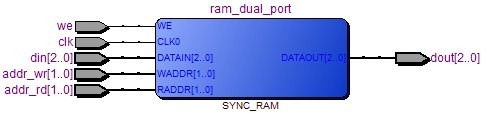
\includegraphics[scale=0.75]{dual_port_RAM}
	\caption{Dual port RAM}
	\label{fig:dual_port_RAM}
\end{figure}

Listing \ref{verilog:dual_port_RAM} is used to implement Fig. \ref{fig:dual_port_RAM}, which is same as Listing \ref{verilog:single_port_RAM} with three changes. First, two address ports are used at Line 25 (i.e. `addr\_rd' and `addr\_wr') instead of one. Next, `addr\_wr' is used to write the data at Line 35; whereas `addr\_rd' data is used to retrieve the data at Line 39. Hence, read and write operation can be performed simultaneously using these two address lines.

Fig. \ref{fig:dual_port_RAM_wave} shows the simulation results for dual port RAM. Here, on the first cursor, `011' is written at address `01'. On next cursor, this value is read along with writing operation as location `10'. Lastly, last two cursor shows that if read and write operation is performed simultaneously on one address e.g. `01', then new data will be available at `dout' port after one clock cycle. 
\begin{figure}[!h]
	\centering
	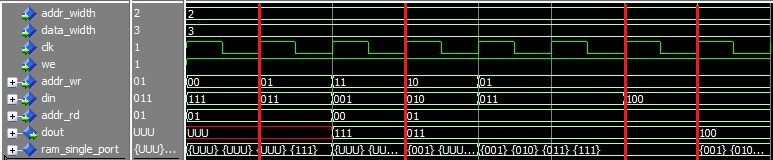
\includegraphics[width=\textwidth]{dual_port_RAM_wave}
	\caption{Simulation results : Dual port RAM (Listing \ref{verilog:dual_port_RAM})}
	\label{fig:dual_port_RAM_wave}
\end{figure}

\lstinputlisting[
language = Verilog,
caption    = {Dual port RAM},
label      = {verilog:dual_port_RAM}
]{dual_port_RAM.v}

\subsection{Visual test : dual port RAM}
Listing \ref{verilog:dual_port_RAM_visualTest} can be use to test the Listing \ref{verilog:dual_port_RAM} on FPGA board. Different combination of switches can be used to store and retrieve the data from RAM. These data will be displayed on LEDs during read operations. 
\lstinputlisting[
language = Verilog,
caption    = {Visual test : dual port RAM},
label      = {verilog:dual_port_RAM_visualTest}
]{dual_port_RAM_visualTest.v}

\section{Read only memory (ROM)}
ROMs are the devices which are used to store information permanently. In this section, ROM is implemented on FPGA to store the display-pattern for seven-segment device, which is explained in Section \ref{sec:sevenSegmentDisplay}. Verilog files required for this example are listed below, 
\begin{enumerate}
	\item ROM\_sevenSegment.v
	\item ROM\_sevenSegment\_visualTest.v
\end{enumerate}

\subsection{ROM implementation using RAM (block ROM)} \label{sec:ROMusingRAM}
Listing \ref{verilog:ROM_sevenSegment} implements the ROM (Lines 27-47), which stores the seven-segment display pattern in it (Lines 30-45). Since the address width is 16 (Line 16), therefore total 16 values can be stored with different addresses (Lines 30-45). Further, 16 addresses can be represented by 4-bits, therefore `addr\_bit' is set to 4 at Line 17. Lastly, total 7 bits are required to represent the number in 7-segment-display, therefore `data\_width' is set to 7 at Line 18.

\lstinputlisting[
language = Verilog,
caption    = {seven segment display pattern stored in ROM},
label      = {verilog:ROM_sevenSegment}
]{ROM_sevenSegment.v}


\subsection{Visual test}
Listing \ref{verilog:ROM_sevenSegment_visualTest} is provided the input `addr' through switches `SW' (Line 20) and then output from Listing \ref{verilog:ROM_sevenSegment} is received to signal `data' (Lines 22-23); which is finally displayed on seven segment display devices (Line 27) and LEDs (Line 28). Here, we can see the switch value on the seven-segment display devices along with the ROM content on LEDs; e.g. if SW value is `011' then `3' will be displayed on seven-segment display and `0000110' will be displayed on LEDs. 
\lstinputlisting[
language = Verilog,
caption    = {Display ROM data on seven segment display and LEDs },
label      = {verilog:ROM_sevenSegment_visualTest}
]{ROM_sevenSegment_visualTest.v}

\section{Queue with first-in first-out functionality}
In this section, Queue is designed with first-in first-out functionality. Verilog files required for this example are listed below, 
\begin{enumerate}
	\item queue.v
	\item queue\_top.v
	\item clockTick.v
	\item modMCounter.v
\end{enumerate}
Note that, `clockTick.v' and `modMCounter.v' are discussed in Chapter \ref{ch:VisualVerification}.

\subsection{Queue design}
Listing \ref{verilog:queue} is the Queue design, which is an example of circular queue. Here, two pointers i.e. Front and rear are used to track the status of the queue i.e. Full or Empty. If read-operation is performed and Front \& Rear pointers are at same location, then queue is empty; whereas if write-operation is performed and Front \& Rear pointers are at same location, then queue is full. Please read the comments for further details.
\lstinputlisting[
language = Verilog,
caption    = {Queue design},
label      = {verilog:queue}
]{queue.v}

\subsection{Visual test}
Listing \ref{verilog:queue_top} is the test circuit for Listing \ref{verilog:queue}. Please read the comments for further details.
\lstinputlisting[
language = Verilog,
caption    = {Visual test of Queue design},
label      = {verilog:queue_top}
]{queue_top.v}
%
